\documentclass[sigconf,nonacm]{acmart}

\usepackage{booktabs}
\usepackage{multirow}
\usepackage{array}
\usepackage{graphicx}
\usepackage{amsmath}
\usepackage{xcolor}
\usepackage{enumitem}
\usepackage{microtype}
\usepackage{balance}

\setlist[itemize]{leftmargin=1.15em, itemsep=1pt, topsep=2pt}
\setlist[enumerate]{leftmargin=1.25em, itemsep=1pt, topsep=2pt}
\setlength{\dbltextfloatsep}{8pt plus 2pt minus 2pt}
\setlength{\textfloatsep}{8pt plus 2pt minus 2pt}
\setlength{\intextsep}{6pt plus 2pt minus 2pt}
\setlength{\abovecaptionskip}{3pt}
\setlength{\belowcaptionskip}{0pt}
\emergencystretch=1.6em

\newcommand{\code}[1]{\texttt{\small #1}}

\title{Beyond Full-Context: Difficulty-Aware Pure-RAG Cascades for High-Precision Scientific Sustainability QA}

\author{[Member 1 Name]}
\authornote{Equal contribution. Replace bracketed placeholders with final team names, student IDs, and agreed role assignments before final submission.}
\affiliation{%
  \institution{The Hong Kong University of Science and Technology (Guangzhou)}
  \department{DSA5020 Final Project (Student ID: [ID-1])}
  \city{Guangzhou}
  \country{China}
}
\email{[member1]@connect.hkust-gz.edu.cn}

\author{[Member 2 Name]}
\authornotemark[1]
\affiliation{%
  \institution{The Hong Kong University of Science and Technology (Guangzhou)}
  \department{DSA5020 Final Project (Student ID: [ID-2])}
  \city{Guangzhou}
  \country{China}
}
\email{[member2]@connect.hkust-gz.edu.cn}

\begin{document}

\begin{abstract}
Question answering over technical sustainability literature demands simultaneous numerical precision ($\pm 0.1\%$ relative tolerance), exact document-level citation grounding, visual chart comprehension, and calibrated abstention on unanswerable queries.
On the WattBot 2025 benchmark (32 scientific PDFs, 641 pages, 41 labeled development and 282 hidden test questions), naive chunk-based retrieval-augmented generation (RAG) fails due to corrupted PDF table extraction, arithmetic rounding errors, and visual blindness, whereas brute-force full-context prompting consumes 689.8k tokens/question without scaling to larger corpora.
We present a fully automated, \emph{zero-full-context} \textbf{Pure-RAG Difficulty-Aware Cascade} built on a single lightweight open model (\code{DeepSeek-V4.1-Flash}).
Our system combines (i)~layout-aware PDF parsing and citation recovery eliminating 100\% of displaced-decimal table corruptions (445$\to$0 rows), (ii)~an agentic tool-using solver (\textsc{Pi Agent v2}) equipped with hybrid search, clean Markdown page reading, a safe Python \code{Decimal} AST arithmetic sandbox bound to cited operands, and explicit reasoning chains, (iii)~an on-demand multimodal visual solver (\code{mode2-only}) rendering candidate PDF pages only when text reasoning abstains, and (iv)~a disagreement- and abstention-triggered gate escalating only 23.4\% of test queries to top-3 document routing.
Across 32 automated Kaggle evaluations, our main Pure-RAG cascade achieves \textbf{0.895 Public / 0.872 Private} at \textbf{79.7k tokens/question}---using \textbf{8.7$\times$ fewer tokens} than raw full-context (0.858 / 0.815) while outperforming the official WattBot 2025 first-place winner KohakuRAG (0.902 / 0.861) by \textbf{+0.011 Private}.
On our Clean v2 index the same cascade essentially matches this Private score (0.871 vs.\ 0.872) at 77.2k tokens/question, while a four-paradigm no-full-context ensemble reaches a project-best \textbf{0.904 Public}---above KohakuRAG's 0.902 Public with zero full-context.
A non-thinking 3-way Pure-RAG consensus further reaches \textbf{0.888 / 0.865} at just \textbf{44.5k tokens/question} (15.5$\times$ cheaper than full-context), and an exploratory full-context-inclusive 5-paradigm ceiling reaches \textbf{0.900 Public / 0.891 Private} (+0.030 Private over first place).
\end{abstract}

\maketitle

\section{Introduction}
\label{sec:intro}

Evaluating the environmental footprint of artificial intelligence---spanning training electricity, water usage, carbon intensity, and hardware lifecycle emissions---requires synthesizing exact quantitative facts across prose, multi-level tables, and charts in scientific papers~\cite{strubell2019energy,patterson2021carbon}.
The Kaggle \textbf{WattBot 2025} competition formalizes this challenge over 32 PDFs (641 pages), providing 41 labeled development questions (\code{train\_QA.csv}) and 282 hidden test questions (\code{test\_Q.csv}).
Submissions are scored by weighted accuracy: normalized answer value correctness (0.75, with strict $\pm 0.1\%$ relative tolerance for numerics and exact \code{[low,high]} interval matching), citation-set Jaccard overlap (0.15), and unanswerable abstention accuracy requiring all five evidence fields to equal \code{is\_blank} (0.10).

Diagnosing baseline chunk RAG~\cite{lewis2020rag} and full-context prompting on WattBot 2025 revealed four concrete failure modes:
\begin{itemize}
  \item \textbf{PDF table and typography corruption.} Default PyMuPDF table extraction corrupts 445 of 835 table rows (53.3\%) with displaced decimals (e.g., \code{4.3} $\to$ \code{43 .}), drops borderless booktabs tables in key papers (\code{strubell2019}, \code{luccioni2025b}), and leaves Unicode ligatures or broken hyphens in 11.1\% of text nodes.
  \item \textbf{Arithmetic and unit-scaling fragility.} Under $\pm 0.1\%$ tolerance, LLM mental arithmetic, premature rounding, and unit-hint mismatches (e.g., millions of liters vs.\ liters) cause avoidable misses even when the right passage is retrieved.
  \item \textbf{Visual blindness on figures.} Pure-text pipelines systematically abstain or guess when exact metrics appear only inside bar charts or plotted curves.
  \item \textbf{Full-context cost collapse.} Concatenating all 32 PDFs consumes 689.8k tokens/question (194.5M total tokens over 282 queries), still drops strict verbatim citations on 20.5\% of answered queries, and cannot scale as corpora grow.
\end{itemize}

\paragraph{Project Contributions.}
Rather than relying on brute-force full-context inputs or proprietary frontier ensembles, we build and benchmark a modular family of automated \textbf{Pure-RAG} pipelines powered by a single lightweight open model (\code{DeepSeek-V4.1-Flash}):
\begin{enumerate}
  \item \textbf{Layout-aware indexing \& zero-token citation recovery:} A hybrid coordinate-plus-Markdown PDF indexer eliminating all 445 displaced-decimal rows and recovering 11 borderless tables, paired with an offline four-tier quote matcher restoring 98.5\% grounded citations.
  \item \textbf{Four orthogonal Pure-RAG paradigms:} Contextual multi-hop hybrid RAG (\textsc{Multi-Hop}, 8.7k tok/q), on-demand visual page reading (\textsc{Multimodal} \code{mode2-only}, 12.8k tok/q), an agentic tool-using solver with a safe \code{Decimal} AST math sandbox and thinking control (\textsc{Pi Agent v2}, 43.2k tok/q), and two-stage card-guided top-3 document routing (\textsc{Doc Routing}, 86.3k tok/q).
  \item \textbf{Difficulty-aware Pure-RAG cascade:} A calibrated arbitration framework pairing \textsc{Pi Agent v2} and \textsc{Multimodal} in Tier~1 and escalating only the 23.4\% disagreed or abstained queries to Tier-2 \textsc{Doc Routing}. With zero full-context, it reaches \textbf{0.895 Public / 0.872 Private} at \textbf{79.7k tok/q}, surpassing first-place KohakuRAG (0.861 Private) at 8.7$\times$ lower cost than full-context.
  \item \textbf{32-submission empirical study:} End-to-end Kaggle evaluation mapping the Accuracy--Token Pareto frontier, $2\times 2$ index/modality ablations, thinking ablations, cross-model comparisons, and error taxonomies.
\end{enumerate}
Individual member contributions are detailed in Section~\ref{sec:contributions}.

\section{Related Work}
\label{sec:related}

Retrieval-Augmented Generation (RAG)~\cite{lewis2020rag} grounds LLM outputs in external corpora via lexical BM25 and dense retrieval fused by Reciprocal Rank Fusion (RRF)~\cite{cormack2009rrf}. Adaptive frameworks add retrieval critique and iterative refinement, including Self-RAG~\cite{asai2024selfrag}, CRAG~\cite{yan2024crag}, MultiHop-RAG~\cite{tang2024multihoprag}, and agentic tool-using RAG~\cite{singh2025agenticrag}. For scientific PDFs, layout-aware parsing~\cite{auer2024docling} and hybrid table--text numerical QA~\cite{zhu2021tatqa} are critical bottlenecks, while VisRAG~\cite{yu2024visrag} shows that visual page retrieval recovers chart evidence missed by text extraction.

Studies comparing RAG with long-context LLMs~\cite{li2024ragvslongcontext} show that hybrid routing captures long-context recall at a fraction of the compute budget. Directly on WattBot 2025, \textbf{KohakuRAG}~\cite{yeh2026kohakurag} won first place (0.902 / 0.861) via a four-level hierarchical document tree, Jina v4 multimodal embeddings, query planning, and multi-model voting with abstention-aware blank filtering. With one lightweight open model and zero full-context inputs, our combination of layout-aware parsing, executable \code{Decimal} sandboxes, on-demand vision, and difficulty-aware cascading surpasses 0.861 Private (0.872 Pure-RAG; 0.891 with full-context ceiling).

\begin{figure*}[t]
  \centering
  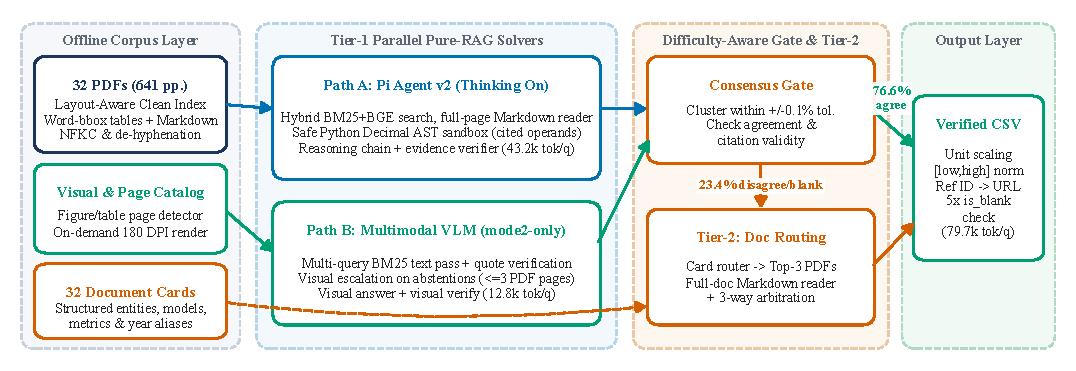
\includegraphics[width=\textwidth]{figures/fig1_architecture.pdf}
  \vspace{-1.6em}
  \caption{End-to-end architecture of our main \textbf{Pure-RAG Difficulty-Aware Cascade} (\code{pi\_on + mode2-only $\to$ doc\_routing}). Tier~1 runs agentic tool-using reasoning with a \code{Decimal} AST sandbox alongside an on-demand visual solver. Only the 23.4\% queries exhibiting inter-path disagreement or abstention escalate to Tier-2 top-3 document routing, eliminating full-context prompting.}
  \label{fig:arch}
  \vspace{-0.7em}
\end{figure*}

\section{System Architecture}
\label{sec:method}

Figure~\ref{fig:arch} depicts our primary \textbf{Pure-RAG Difficulty-Aware Cascade}. Every stage is automated in Python and Node.js, writes per-question JSONL traces with exact API token usage, and validates outputs against schema, question order, metadata URLs, and the five \code{is\_blank} abstention fields via \code{wattbot verify}.

\subsection{Layout-Aware Indexing \& Citation Recovery}
\label{sec:indexing}

\paragraph{Clean v2 Index (\code{wattbot.clean\_index}).}
To fix the 53.3\% table corruption rate in the baseline v1 index, we assign PDF words inside detected \code{find\_tables()} cells by word-center coordinates rather than raw stream order, preserving decimal points and multi-level headers with units. For borderless booktabs papers (\code{strubell2019}, \code{luccioni2025b}), we fall back to \code{pymupdf4llm} Markdown tables. Each table emits both \code{table\_row} nodes and multi-row \code{table\_block} nodes (183 blocks) with nearby captions; body text applies Unicode NFKC normalization and prefix-aware line-wrap de-hyphenation.

\paragraph{Offline Citation Recovery (\code{wattbot.citation\_recovery}).}
Strict substring quote checks drop valid citations when OCR whitespace or ellipses differ from source text. Our four-tier matcher (\code{exact}, \code{token\_span}, \code{ellipsis\_segments}, and \code{token\_lcs} with a numeric-token guard) searches hierarchically across \code{same\_page}, \code{adjacent\_page}, \code{same\_doc}, and \code{corpus\_unique} at zero LLM token cost.

\subsection{Tier-1 Path A: \textsc{Pi Agent v2} with \code{Decimal} AST Sandbox}
\label{sec:piv2}

Built on Pi Agent Core (\code{pi\_rag/agent\_v2.mjs}) bridged to Python tool executors (\code{wattbot/pi\_agent\_v2.py}), \textsc{Pi Agent v2} executes an iterative tool loop (up to 8 parallel tool calls/question):
\begin{itemize}
  \item \code{list\_documents()} lists all 32 papers for cross-document lookup.
  \item \code{search\_corpus(query, ref\_id?, top\_k?)} fuses BM25 and dense embeddings (\code{bge-small-en-v1.5}~\cite{xiao2024bge}) via RRF, optionally scoped to one document.
  \item \code{read\_page(ref\_id, page)} renders clean Markdown tables and full page text directly from the source PDF.
  \item \code{eval\_math(expression, named\_operands, result\_unit)} evaluates arithmetic in a restricted Python \code{ast} sandbox with exact \code{Decimal} math. Corpus numbers bind to a \code{node\_id} and quote (or prior \code{calculation\_id}); physical constants are pre-registered, and answers must match the bound calculation after unit conversion.
  \item \code{submit\_answer(...)} enforces boolean semantics (\code{1} supported, \code{0} contradicted, \code{is\_blank} only if unanswerable), scales \code{unit\_hint} canonically, and runs an LLM evidence verifier.
\end{itemize}
A controlled \code{--thinking} switch toggles \code{enable\_thinking} in the API request while preserving \code{reasoning\_content} across turns and logging \code{reasoning\_tokens}.

\subsection{Tier-1 Path B: On-Demand Multimodal Visual Solver}
\label{sec:multimodal}

To avoid vision-token overhead on text-answerable questions, \code{wattbot.multimodal} (\code{mode2-only}) first catalogs figure/table pages offline across all 32 PDFs. At inference it runs a fast multi-query BM25 pass with quote verification and escalates visually \emph{only} on abstentions: up to 3 pages are rendered at 180~DPI and sent to the vision-capable campus model with page text, then visually verified. Only 39 of 282 test queries (13.8\%) trigger vision (277 images total), keeping mean cost at 12.8k tok/q.

\subsection{Tier-2 Escalation: Document Routing \& Arbitration}
\label{sec:cascade}

\paragraph{Two-Stage Document Routing (\code{wattbot.doc\_routing}).}
Instead of sending all 32 PDFs (687k tokens), we pre-build 32 structured \emph{Document Cards} (242k tokens once) summarizing each paper's entities, authors, year aliases, models, hardware, and metrics. Stage~1 routes against all 32 cards to pick the Top-3 papers; Stage~2 reads only those 3 papers in clean Markdown (86.3k tok/q---8.0$\times$ cheaper than full-context).

\paragraph{Difficulty-Aware Cascade \& Consensus (\code{wattbot.ensemble}).}
Our arbitration engine clusters non-blank answers via complete-linkage equivalence within $\pm 0.1\%$ numeric tolerance after canonicalizing \code{[low,high]} intervals and booleans, weighting each candidate by citation validity, verifier outcomes, and executable \code{calculation\_binding}.
In our \textbf{main Pure-RAG cascade}, Tier~1 runs \textsc{Pi Agent v2} (\code{thinking=true}) and \textsc{Multimodal} (\code{mode2-only}) in parallel. If both agree with valid citations (76.6\% of test queries), we accept immediately. Only on the remaining \textbf{23.4\%} (66/282) queries with disagreement (30) or abstention (36) does the gate invoke Tier-2 \textsc{Doc Routing} and arbitrate across all three paths via majority citation reconciliation.

For ultra-low-budget deployment, \textbf{Multi-Hop Contextual Hybrid RAG} (\code{wattbot.multihop\_rag}, 8.7k tok/q) pairs \code{pymupdf4llm} contextual chunks, \code{bge-small-en-v1.5} + BM25 RRF, a \code{jina-reranker} cross-encoder, and iterative missing-fact retrieval~\cite{yeh2026kohakurag}.

\section{Experimental Setup and Main Results}
\label{sec:experiments}

\subsection{Experimental Protocol}
All primary experiments run on the HKUST(GZ) AIGC campus gateway with \code{DeepSeek-V4.1-Flash} (\code{temperature=0}, JSON-mode outputs). For cross-model evaluation, we also test \code{DeepSeek-V4-Pro} and \code{Qwen3.8-27B} on the v1 index. Every test CSV passes \code{wattbot verify} (282-row ID alignment, valid metadata URLs, 5-field \code{is\_blank} checks) and is scored on Kaggle's Public and Private splits. Token usage is aggregated from server-reported API \code{usage} fields (\code{prompt\_tokens} + \code{completion\_tokens}).

\begin{table*}[t]
  \centering
  \caption{Evaluation across baselines, single-path RAG systems, Pure-RAG cascades/ensembles, and Full-Context upper bounds on WattBot 2025 (41 train / 282 Kaggle test questions). All primary methods use a single model (\code{DeepSeek-V4.1-Flash}) unless noted. Bold marks the best score per category; \textbf{Main System} uses zero full-context.}
  \label{tab:main}
  \footnotesize
  \setlength{\tabcolsep}{4.5pt}
  \begin{tabular}{@{}llrrrrrr@{}}
    \toprule
    \textbf{Category} & \textbf{System / Configuration} & \textbf{Train (41q)} & \textbf{Ans / Blank} & \textbf{Mean Tok/Q} & \textbf{vs.\ FC} & \textbf{Public} & \textbf{Private} \\
    \midrule
    \multirow{4}{*}{Baselines}
      & Minimal all-\code{is\_blank} smoke fallback & --- & 0 / 282 & 0 & --- & 0.138 & 0.175 \\
      & Direct LLM (Closed-book, Flash) & 0.3354 & 134 / 148 & 246 & 0.0004$\times$ & 0.286 & 0.419 \\
      & Baseline v1 Chunk RAG (BM25, Flash, norm.) & 0.7604 & 236 / 46 & 11,001 & 0.016$\times$ & 0.814 & 0.750 \\
      & Full-Context Baseline (raw v1, Flash) & 0.7988 & 259 / 23 & 689,804 & 1.00$\times$ & 0.858 & 0.815 \\
    \midrule
    \multirow{2}{*}{Cross-Model}
      & v1 Chunk RAG (\code{Qwen3.8-27B}) & 0.7543 & 230 / 52 & 12,764 & 0.019$\times$ & 0.830 & 0.694 \\
      & v1 Chunk RAG (\code{DeepSeek-V4-Pro}) & 0.7713 & 225 / 57 & 12,523 & 0.018$\times$ & 0.781 & 0.720 \\
    \midrule
    \multirow{8}{*}{\shortstack[l]{Single-Path\\Systems\\(Flash)}}
      & Pi Agent v1 (tool-using baseline) & 0.7628 & 226 / 56 & 10,786 & 0.016$\times$ & 0.785 & 0.735 \\
      & Clean-index v2 Text-only RAG (Stage 1) & 0.8262 & 241 / 41 & $\sim$9,301$^\dagger$ & 0.013$\times$ & 0.848 & 0.768 \\
      & Standalone Multimodal (\code{mode2-only}, v1) & 0.8354 & 258 / 24 & 12,848 & 0.019$\times$ & 0.854 & 0.807 \\
      & Clean-index v2 RAG + Multimodal Cascade & 0.8530 & 259 / 23 & 15,292 & 0.022$\times$ & 0.858 & 0.815 \\
      & Pi Agent v2 (\code{thinking=false}) & 0.8628 & 253 / 29 & 22,929 & 0.033$\times$ & 0.873 & 0.818 \\
      & Multi-hop Contextual Hybrid RAG & 0.7988 & 249 / 33 & \textbf{8,708} & \textbf{0.013$\times$} & 0.852 & 0.825 \\
      & Two-Stage Document Routing (Top-3) & \textbf{0.8951} & 258 / 24 & 86,253 & 0.125$\times$ & \textbf{0.885} & 0.841 \\
      & Pi Agent v2 (\code{thinking=true}) & 0.8866 & 253 / 29 & 43,182 & 0.063$\times$ & 0.870 & \textbf{0.854} \\
    \midrule
    \multirow{7}{*}{\shortstack[l]{\textbf{Pure-RAG}\\Cascades \&\\Ensembles\\(Zero FC)}}
      & 3-Way Consensus (\code{mhop+mm+pi\_off}, no Think) & 0.8982 & 267 / 15 & \textbf{44,485} & \textbf{0.064$\times$} & 0.888 & 0.865 \\
      & Cascade (\code{mhop+v2cas $\to$ pi\_on}, 20.6\% esc.) & 0.9171 & 265 / 17 & 54,273 & 0.079$\times$ & 0.879 & 0.864 \\
      & 3-Way Consensus (\code{mhop+v2cas+pi\_on}) & 0.9171 & 265 / 17 & 67,182 & 0.097$\times$ & 0.880 & 0.865 \\
      & Pure-RAG Casc.\ v2 (\code{pi\_on+mm $\to$ doc}, 24.1\% esc.) & 0.9012 & 268 / 14 & 77,228 & 0.112$\times$ & 0.895 & 0.871 \\
      & \textbf{Main: Cascade (\code{pi\_on+mm $\to$ doc}, 23.4\% esc.)} & 0.8970 & 267 / 15 & 79,711 & 0.116$\times$ & 0.895 & \textbf{0.872} \\
      & 4-Paradigm Consensus (\code{pi\_on+doc+mhop+mm}, BF) & \textbf{0.9171} & 267 / 15 & 150,991 & 0.219$\times$ & 0.896 & \textbf{0.872} \\
      & 4-Paradigm No-FC (\code{Clean v2} \textsc{Pi} v2, BF) & --- & 268 / 14 & 148,014 & 0.215$\times$ & \textbf{0.904} & 0.864 \\
    \midrule
    \multirow{5}{*}{\shortstack[l]{Full-Context\\Reference\\Upper Bounds}}
      & Full-Context + Offline Citation Recovery & 0.8290 & 259 / 23 & 689,804 & 1.00$\times$ & 0.883 & 0.837 \\
      & Cascade: v1 RAG $\to$ Full-Context (16.3\% esc.) & 0.8134 & 262 / 20 & 125,557 & 0.182$\times$ & 0.868 & 0.845 \\
      & 7-Run Correlated Consensus (\code{+pi\_off+v2cas}, BF) & 0.8988 & 268 / 14 & 879,016 & 1.27$\times$ & 0.896 & 0.865 \\
      & 5-Paradigm Consensus (\code{pi\_on+doc+fc+mhop+mm}, BF) & 0.9024 & 268 / 14 & 840,795 & 1.22$\times$ & \textbf{0.900} & 0.888 \\
      & 5-Paradigm Quorum (\code{q0.5}) $\to$ Multimodal Cascade & 0.9018 & 266 / 16 & 840,795 & 1.22$\times$ & 0.896 & \textbf{0.891} \\
    \midrule
    \textit{External Ref.} & \textit{KohakuRAG (WattBot 2025 1st Place~\cite{yeh2026kohakurag})} & --- & --- & --- & --- & \textit{0.902} & \textit{0.861} \\
    \bottomrule
  \end{tabular}
  \vspace{-0.3em}
  \par\raggedright\scriptsize $^\dagger$Stage-1 text-only mean tokens measured on the 41-question live cascade trace (9,301 tok/q); test cascade total is 15,292 tok/q. BF = abstention-aware blank filtering (\code{q0/s0}).
  \vspace{-0.6em}
\end{table*}

\subsection{Main Quantitative Results}
Table~\ref{tab:main} summarizes 26 representative configurations from our 32 Kaggle evaluations, plus the external KohakuRAG reference (full log in \code{docs/kaggle-test-results.md}), and Figure~\ref{fig:pareto} plots the Accuracy--Token Pareto frontier on the Private leaderboard:

\begin{figure}[t]
  \centering
  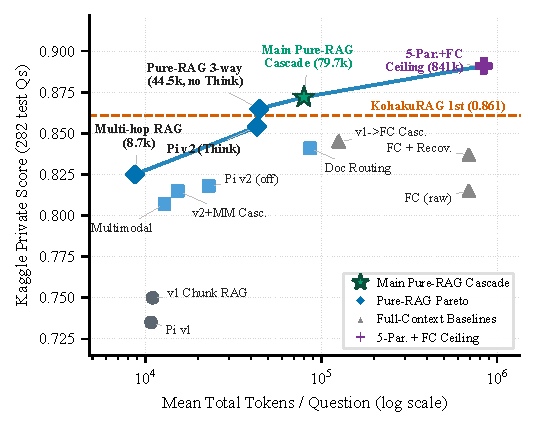
\includegraphics[width=\columnwidth]{figures/fig2_pareto.pdf}
  \vspace{-1.5em}
  \caption{Accuracy--Token Pareto frontier on the 282-question Kaggle Private leaderboard (zoomed to 0.715--0.922; lower baselines Direct 0.419 @ 246 tok/q and Minimal 0.175 @ 0 omitted for clarity). Pure-RAG strictly dominates Full-Context and beats KohakuRAG (0.861) from 44.5k tok/q onward.}
  \label{fig:pareto}
  \vspace{-0.8em}
\end{figure}

\paragraph{1. Pure-RAG strictly Pareto-dominates Full-Context.}
Raw Full-Context burns 689.8k tok/q for 0.858 Public / 0.815 Private (0.883 / 0.837 after citation recovery). By contrast, \textsc{Multi-Hop} (\textbf{8.7k tok/q}, 79$\times$ cheaper) reaches \textbf{0.825 Private}, beating raw Full-Context. Our strongest single-path system, \textsc{Pi Agent v2} (\code{thinking=true}, \textbf{43.2k tok/q}, 16$\times$ cheaper), achieves \textbf{0.870 Public / 0.854 Private}, within 0.007 of multi-model KohakuRAG (0.861). \textsc{Doc Routing} (86.3k tok/q, 8$\times$ cheaper) achieves the highest single-path Public score (\textbf{0.885}) and 0.841 Private.

\paragraph{2. Main Pure-RAG Cascade surpasses KohakuRAG without Full-Context.}
Our main system---\code{Pi v2 (thinking=true) + Multimodal mode2-only $\to$ Doc Routing} on the 23.4\% disagreed/abstained queries---achieves \textbf{0.895 Public / 0.872 Private} at \textbf{79.7k tok/q}. It beats KohakuRAG's Private score (0.861) by \textbf{+0.011}, matches the 151k tok/q 4-paradigm consensus (0.896 / 0.872) at half the tokens, and costs less than running \textsc{Doc Routing} alone (86.3k tok/q). Rebuilt end-to-end on Clean v2 with the same gate, it keeps \textbf{0.895 Public / 0.871 Private} at \textbf{77.2k tok/q} (24.1\% escalation).

\paragraph{3. Ultra-low-cost Pure-RAG without Thinking or Document Routing.}
Combining our three lightest orthogonal RAG paths (\textsc{Multi-Hop} 8.7k + \textsc{Multimodal} 12.8k + \textsc{Pi v2 thinking=false} 22.9k) requires just \textbf{44.5k tok/q} (15.5$\times$ cheaper than Full-Context) without thinking or full-document reads, yet achieves \textbf{0.888 Public / 0.865 Private}---exceeding KohakuRAG (0.861) and well suited for live demos.

\paragraph{4. Full-Context exploratory upper bound.}
When compute is unconstrained, adding citation-recovered Full-Context into an orthogonal 5-paradigm ensemble yields \textbf{0.900 Public / 0.888 Private} under blank filtering and \textbf{0.896 Public / 0.891 Private} (+0.030 Private over KohakuRAG) under quorum voting (\code{q0.5}) followed by multimodal fallback on the 21 remaining abstentions.

\begin{figure*}[t]
  \centering
  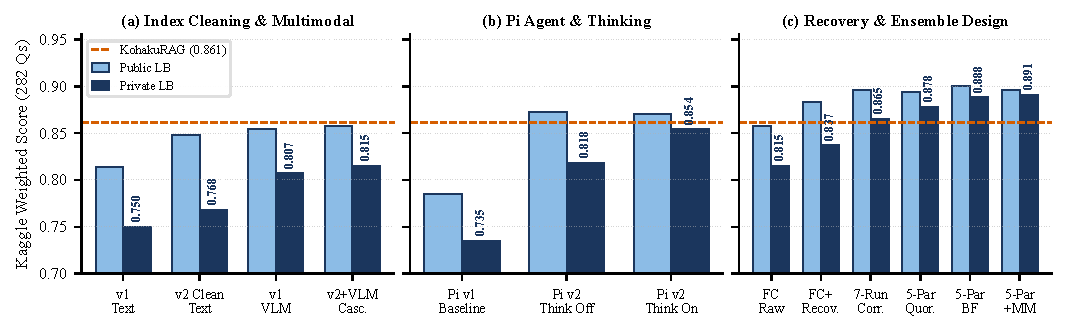
\includegraphics[width=\textwidth]{figures/fig3_ablations.pdf}
  \vspace{-1.6em}
  \caption{Controlled test-set ablations on Kaggle Public and Private leaderboards (282 Qs): (a)~2$\times$2 index cleaning $\times$ multimodal cascade; (b)~\textsc{Pi Agent} v1$\to$v2 and thinking toggle; (c)~offline citation recovery, paradigm orthogonality (7-run correlated vs.\ 5-paradigm), and quorum + multimodal calibration.}
  \label{fig:ablations}
  \vspace{-0.7em}
\end{figure*}

\begin{figure*}[t]
  \centering
  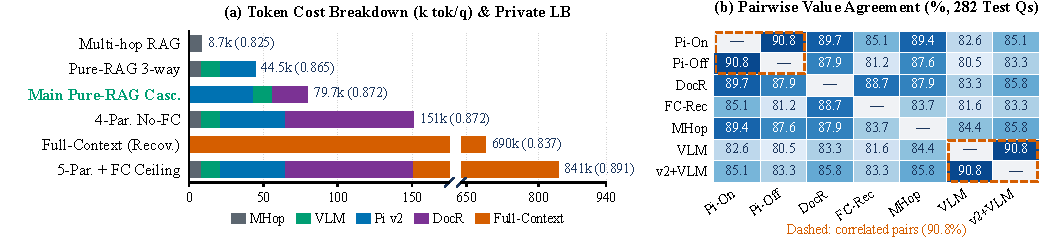
\includegraphics[width=0.97\textwidth]{figures/fig4_cost_diversity.pdf}
  \caption{(a)~Stage-wise token cost (broken axis): Main Pure-RAG Cascade (79.7k) and 3-way consensus (44.5k) remove the 82\% Full-Context bottleneck while surpassing KohakuRAG (0.861); (b)~pairwise test agreement (282 Qs) exposing the two 90.8\% correlated pairs.}
  \label{fig:costdiv}
  \vspace{-0.8em}
\end{figure*}

\section{Ablation, Cost, and Error Analysis}
\label{sec:analysis}

\subsection{Index Cleaning, Multimodal 2$\times$2, and Citation Recovery}
Table~\ref{tab:index} audits our v2 clean indexer, and Figure~\ref{fig:ablations}(a) shows the 2$\times$2 test ablation under identical \code{DeepSeek-V4.1-Flash} BM25 settings:
\begin{itemize}
  \item \textbf{v1 $\to$ v2 Clean Index:} Eliminating all 445 displaced-decimal rows, 497 ligatures, and 1,317 broken hyphens lifts pure-text RAG from 0.814 / 0.750 to \textbf{0.848 / 0.768} (+0.034 Pub, +0.018 Priv) while cutting train tokens 24.8\% (12.2k $\to$ 9.2k).
  \item \textbf{Multimodal 2$\times$2 Gain:} Adding on-demand vision lifts v1 text to 0.854 / 0.807 (+0.057 Priv); cascading multimodal fallback after Clean v2 text abstentions (41/282 escalations, 18 recovered) reaches \textbf{0.858 / 0.815} (+0.047 Priv over Clean v2 text).
  \item \textbf{Zero-Token Citation Recovery:} Replaying our four-tier quote matcher over the Full-Context test trace restores citations on 49 answered queries (206/259 $\to$ 255/259, 98.5\%), lifting scores from 0.858 / 0.815 to \textbf{0.883 / 0.837} (+0.025 Pub, +0.022 Priv) with zero LLM calls (Figure~\ref{fig:ablations}(c)).
\end{itemize}

\begin{table}[t]
  \centering
  \caption{Corpus index audit: v1 baseline vs.\ v2 clean index (32 PDFs, 641 pages).}
  \label{tab:index}
  \footnotesize
  \setlength{\tabcolsep}{4.5pt}
  \begin{tabular}{@{}lrrr@{}}
    \toprule
    \textbf{Index Quality Metric} & \textbf{v1 Index} & \textbf{v2 Clean} & \textbf{Delta} \\
    \midrule
    Extracted tables (docs w/ tables) & 131 (27/32) & 142 (29/32) & +11 tables \\
    Multi-row \code{table\_block} nodes & 0 & 183 & +183 \\
    Displaced-decimal rows (\code{\textbackslash d\textbackslash s+\textbackslash .}) & 445 / 835 & \textbf{0 / 819} & $-100.0\%$ \\
    Text nodes with Unicode ligatures & 497 / 16,372 & \textbf{0 / 16,372} & $-100.0\%$ \\
    Text nodes with broken hyphens & 1,317 / 16,372 & \textbf{0 / 16,372} & $-100.0\%$ \\
    \bottomrule
  \end{tabular}
  \vspace{-0.8em}
\end{table}

\subsection{\textsc{Pi Agent} Evolution and Thinking Ablation}
Figure~\ref{fig:ablations}(b) isolates the agentic toolchain and thinking gains on the v1 index:
\begin{itemize}
  \item \textbf{\textsc{Pi v1} $\to$ \textsc{Pi v2} (\code{thinking=false}):} Adding Markdown \code{read\_page}, hybrid BM25+BGE search, parallel tool calls, and the operand-bound \code{Decimal} AST sandbox lifts Kaggle scores from 0.785 / 0.735 to \textbf{0.873 / 0.818} (+0.088 Pub, +0.083 Priv) while halving abstentions (56 $\to$ 29).
  \item \textbf{Controlled Thinking Ablation (\code{false} $\to$ \code{true}):} Enabling thinking adds 161,629 reasoning tokens over 282 queries (22.9k $\to$ 43.2k tok/q) and nearly doubles active search (\code{search\_corpus} 219 $\to$ 428; \code{read\_page} 58 $\to$ 95), driving a \textbf{+0.036 Private} jump (0.818 $\to$ \textbf{0.854}).
\end{itemize}

\subsection{Token Cost Decomposition \& Efficiency Analysis}
Figure~\ref{fig:costdiv}(a) decomposes per-question token budgets across our Pure-RAG systems and the 5-paradigm ensemble (840,795 tok/q, 237.1M total tokens over 282 test questions):
\begin{itemize}
  \item \textbf{Full-Context consumes 82.0\% (194.5M tokens)}, resending 687k tokens for all 282 test queries.
  \item \textbf{Doc Routing (10.3\%, 24.3M)} sends 32 cards ($\sim$26k tok/q) plus Top-3 full papers ($\sim$60k tok/q).
  \item \textbf{\textsc{Pi v2 Thinking} (5.1\%, 12.2M)} spends 97.3\% on prompt tokens from multi-turn growth (3.3 calls/q); \textsc{Multimodal} (1.5\%) and \textsc{Multi-Hop} (1.0\%) stay compact.
\end{itemize}
Our Pure-RAG cascade (\code{pi\_on + mm $\to$ doc\_routing}) cuts gross token volume by \textbf{90.5\%} vs.\ the 5-paradigm ensemble (841k$\to$79.7k) and \textbf{88.4\%} vs.\ Full-Context (690k$\to$79.7k), beating it by +0.035 to +0.057 Private.

\subsection{Cross-Model Comparison \& Paradigm Orthogonality}
On the v1 index, \code{DeepSeek-V4.1-Flash} (0.814 / 0.750) outperforms \code{DeepSeek-V4-Pro} (0.781 / 0.720) and \code{Qwen3.8-27B} (0.830 / 0.694) on Private LB, confirming that retrieval, parsing, and verification engineering dominate raw model scale.
Figure~\ref{fig:ablations}(c) and Figure~\ref{fig:costdiv}(b) highlight two ensemble laws:
(1)~\textbf{Orthogonality beats correlation:} As shown in Figure~\ref{fig:costdiv}(b), the two correlated pairs (\code{Pi-On}/\code{Pi-Off} and \code{VLM}/\code{v2+VLM}) agree on \textbf{90.8\%} of test questions, whereas orthogonal pairs (e.g., \code{Pi-On}/\code{VLM} at 82.6\%, \code{FC-Rec}/\code{VLM} at 81.6\%) diverge substantially. Adding these correlated voters into a 7-run ensemble drops Private LB from \textbf{0.888} (5 orthogonal paradigms) to \textbf{0.865} ($-0.023$).
(2)~\textbf{Quorum + Multimodal cascade balances abstention and vision:} Quorum (\code{q0.5}, 0.878) blocks lone text hallucinations on unanswerable queries but suppresses chart answers; blank filtering (\code{q0/s0}, 0.888) recovers charts with slight hallucination risk; cascading only the 21 remaining \code{q0.5} abstentions to \code{mode2-only} (5 recoveries) reaches \textbf{0.891 Private}. The reversal is quorum arithmetic: an even 4-voter pool makes \code{q0.5} demand $\ge$2 agreeing voters, suppressing valid minority answers more sharply than an odd 5-voter pool, so 4-way BF (0.872) beats 4-way quorum+MM (0.865) while 5-way quorum+MM (0.891) beats 5-way BF (0.888).

\subsection{Residual Error Taxonomy and Index Transfer}
Error inspection reveals four residual failure modes:
(1)~\emph{Chart-only metrics:} Test \code{q015}, \code{q189}, \code{q317} and train \code{q215} (\code{schwartz2019} Fig.~2) are abstained by all top text systems yet solved by \code{mode2-only};
(2)~\emph{Prose vs.\ table precision:} On \code{q124}, prose rounds ``5.4M liters'' while Table~1 states ``5.439M'' (outside $\pm 0.1\%$);
(3)~\emph{Integer vs.\ exact arithmetic:} On \code{q280}, dividing hours by 24 gives \code{13.0208} vs.\ gold \code{13} days (0.16\% gap);
(4)~\emph{Index cleaning is paradigm-dependent:} Moving \textsc{Pi v2} to Clean v2 cuts tokens 6.9\% (43.2k$\to$40.2k) and lifts Public 0.870$\to$0.879, while the cascade holds Private at 0.871 (vs.\ 0.872) and the 4-paradigm no-FC ensemble reaches a project-best \textbf{0.904 Public}. Because \code{read\_page()} already renders clean \code{pymupdf4llm} Markdown from the PDF, Clean v2's table repair largely duplicates that reader: single-path Private is slightly lower (0.841; on \code{q124} prose outranks the exact table cell) and Clean v2 benefits Chunk RAG most (+0.018).

\paragraph{Limitations.}
Ablation deltas near 0.005 on our 41-question development set are within calibration noise, and all reported systems share one open model family (\code{DeepSeek-V4.1-Flash}), so cross-family generality is untested. Document Cards currently assume a 32-paper corpus; scaling to thousands of papers would require hierarchical card routing (corpus $\to$ field $\to$ venue $\to$ paper) to keep Stage-1 routing linear. Finally, the abstention and escalation thresholds are tuned on 41 train questions and may drift on a new corpus.

\section{Team Contributions \& Reproducibility}
\label{sec:contributions}

\subsection{Individual Contributions}
Our two-member team divided the engineering tracks evenly with joint ownership of experimental design, Kaggle evaluation, and report writing (Table~\ref{tab:contrib}).

\begin{table}[t]
  \centering
  \caption{Individual contributions of each team member. (Replace bracketed placeholders with final names/roles.)}
  \label{tab:contrib}
  \footnotesize
  \setlength{\tabcolsep}{4pt}
  \begin{tabular}{@{} >{\raggedright\arraybackslash}p{0.24\columnwidth} p{0.71\columnwidth} @{}}
    \toprule
    \textbf{Team Member} & \textbf{Primary Responsibilities \& Deliverables} \\
    \midrule
    \textbf{[Member 1 Name]} \newline (\code{[ID-1]}, 50\%) &
      Data ingestion, Clean v2 layout-aware indexing (\code{clean\_index.py}), offline four-tier citation recovery (\code{citation\_recovery.py}), baseline RAG / Direct / Full-Context pipelines, two-stage Document Routing (\code{doc\_routing.py}), trace/schema verification, and Sec.~3.1, 3.4, 5.1, 5.3. \\
    \midrule
    \textbf{[Member 2 Name]} \newline (\code{[ID-2]}, 50\%) &
      Agentic \textsc{Pi Agent v1/v2} with safe Python \code{Decimal} AST sandbox \& thinking ablation (\code{pi\_agent\_v2.py}, \code{agent\_v2.mjs}), Multimodal VLM (\code{multimodal.py}), Multi-Hop contextual RAG (\code{multihop\_rag.py}), cross-model \& cascade ensemble (\code{ensemble.py}), Kaggle sweeps, figures, and Sec.~3.2, 3.3, 4, 5.2, 5.4--5.5. \\
    \bottomrule
  \end{tabular}
  \vspace{-0.8em}
\end{table}

\subsection{Reproducibility and Package Organization}
The submission ZIP contains the top-level report PDF; \code{code/} (\code{wattbot/}, \code{pi\_rag/}, the zero-dependency interactive \code{demo/}, \code{scripts/}, \code{tests/}, \code{docs/}, and an MIT \code{LICENSE}); \code{dataset/} (raw CSVs and the 32 PDFs under \code{docs/}); verified \code{demo\_outputs/} CSVs; and \code{report/} \LaTeX{} sources. All \textbf{208/208} unit tests pass (\code{unittest discover -s tests}). The full system runs online via \code{python -m wattbot} \code{pure-rag-cascade}, which executes both Tier-1 solvers, applies the consensus gate, and invokes Tier-2 \code{doc\_routing} \emph{only} on escalated queries. The equivalent manual replay takes four steps:
(1)~\code{wattbot index}, \code{clean\_index}, and \code{doc\_routing build};
(2)~\code{pi\_agent\_v2} \code{--split test --thinking true} and \code{multimodal run --mode mode2-only};
(3)~\code{doc\_routing run --top-docs 3};
(4)~\code{ensemble cascade} (\code{pi\_on+mm $\to$ doc}) and \code{wattbot verify}.
For live presentation, \code{demo/app.py} serves an offline Trace Explorer (saved traces and cited PDF pages, no API key) plus a Live Q\&A mode using only the Python standard library.

\section{Conclusion}
\label{sec:conclusion}

High-precision scientific QA does not require full-context prompting or proprietary model ensembles. By fixing PDF table corruption, grounding math in a cited \code{Decimal} AST sandbox, invoking page vision on demand, and escalating only disagreed or abstained queries to top-3 document routing, our \textbf{Pure-RAG Cascade} reaches \textbf{0.895 Public / 0.872 Private} at \textbf{79.7k tok/q} on one lightweight open model (\code{DeepSeek-V4.1-Flash})---8.7$\times$ cheaper than full-context and +0.011 Private above KohakuRAG (0.861); on Clean v2, a 4-paradigm ensemble reaches a project-best \textbf{0.904 Public}. Future work will add native multimodal embeddings, hierarchical card routing for corpora far larger than 32 papers, and cross-model difficulty-aware ensembles.

\bibliographystyle{ACM-Reference-Format}
\balance
\bibliography{references}

\end{document}
